\section{Computational Study}\label{sec:r51-study}
Table~\ref{tab:r51-regimes} separates the proved regimes before comparing implementations. All inputs below are synthetic rational data, not estimated contracts or operational observations. The protocol fixes generators, seeds, insertion paths, node allowances, price-trial allowances, and envelope resolutions before local execution. Its immutable file and hash identify this experiment; it was not a remotely preregistered experiment. Timing comparisons below use the same recorded execution environment. Earlier timings are not relabeled as matched measurements.

\subsection{Difficult instances and interruption certificates}
We retain the six distinct 12-history, nine-candidate, three-symbol instances underlying the preceding multi-class stress requests. Seventy-two new timed requests cross node allowances of 1, 7, 31, and 127 with 0, 2, and 5 local price trials. Six additional completion runs receive larger allowances. Table~\ref{tab:r51-hard} compares their exact final intervals with the old group-box gaps. All six completion runs close at zero rational width, using at most 21 visited nodes. Their values agree with the previously available exhaustive references: those values are not newly discovered optima. The new evidence is closure by a compact, independently checked selected-prefix cover rather than unresolved group-mean boxes or full book enumeration.

Figure~\ref{fig:r51-nodes} reports the largest certified absolute gap across these six unchanged inputs at each node allowance. It retains every requested allowance, including unsuccessful early interruptions. A positive-width interval is not an exact solution, even when its width meets a requested tolerance. The global endpoints, rather than rounded display values or numerical statuses, determine all exactness labels.
\begin{figure}[t]\centering
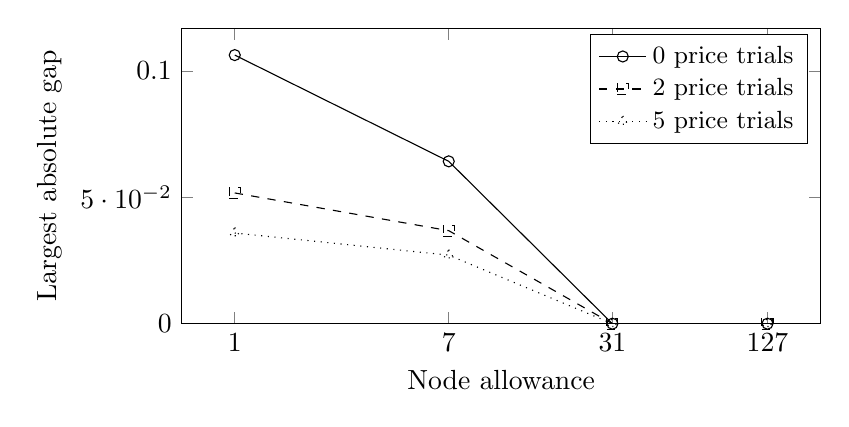
\begin{tikzpicture}\begin{axis}[width=.8\textwidth,height=2.1in,xmode=log,log basis x=2,xlabel={Node allowance},ylabel={Largest absolute gap},legend style={at={(.98,.98)},anchor=north east,font=\small},ymin=0,xtick={1,7,31,127},xticklabels={1,7,31,127}]
\addplot[solid,mark=o] coordinates {(1,0.10625) (7,0.0642181705229) (31,0) (127,0)};\addlegendentry{0 price trials}
\addplot[dashed,mark=square] coordinates {(1,0.0517181705229) (7,0.036796875) (31,0) (127,0)};\addlegendentry{2 price trials}
\addplot[dotted,mark=triangle] coordinates {(1,0.0358746189024) (7,0.0271215820313) (31,0) (127,0)};\addlegendentry{5 price trials}
\end{axis}\end{tikzpicture}
\caption{Node-budget and price sensitivity on the six fixed historical stress inputs. The vertical axis is the maximum rational interval width, converted to a display decimal only after verification. All requested budgets, including positive-width interruptions, contribute to the plot.}\label{fig:r51-nodes}
\end{figure}


\subsection{Nontrivial common eligibility and matched class counts}
The 20 strict-prefix instances in Table~\ref{tab:r51-strict} and the companion test common eligibility without making every candidate eligible. The catalog is nonuniform. All ceilings are distinct points strictly inside one interior catalog gap; an entire candidate suffix is ineligible. Caps, probabilities, curvatures, and zero-cost branches remain individual. Promise fractions one third and nine tenths test interior allocations, and the additional 33-level cases vary budgets two and four. Every case is solved exactly by the inherited one-class pooled oracle, including 1,024-history cases. The former all-ceilings-equal-one family remains available as an arithmetic scaling experiment, not evidence of threshold robustness.

Table~\ref{tab:r51-matched} holds the 16-history, 17-candidate, three-symbol primitives fixed while changing only the ceilings to obtain one through eight classes. Forty-eight requests cross those class counts with three node allowances and two price settings. All 127-node requests close exactly. Local prices reduce nodes in each paired row, but their additional arithmetic makes every displayed priced run slower. Thus fewer nodes are not evidence of lower wall time, and neither these small-class data nor the common-prefix scale experiment establish a universal runtime ranking.

\subsection{Refinement, screening, and safety boundaries}
Table~\ref{tab:r51-refine} follows six stages of candidate insertion with two opening-charge schedules, each with screening enabled and disabled. In the high-charge path, insertions raise the raw class count from one to four without changing the optimum. Exact screening removes every inserted candidate, retains one active class, and closes at the root throughout. Without screening the search still certifies the same optimum, but visits more nodes. In the low-charge path, new candidates can improve the optimum. This comparison separates harmless class splitting from genuine expansion of the feasible design choices; it does not assume that every newly introduced candidate is irrelevant.

Twelve additional boundary requests place selected subsets of eight thresholds just below or just above a candidate. Three perturbation magnitudes range from $10^{-2}$ to $10^{-6}$. Within a fixed signature cell their exact values agree, while a changed eligible set can change the value. The one-history discontinuity in Section~\ref{sec:r51-robust} is checked separately. These experiments test the stability statements and do not replace a missing calibrated safety model.

\subsection{Direct optimization and certificate economics}
Table~\ref{tab:r51-mip} reports the direct mixed-integer formulation on the six difficult inputs and three matched-class inputs. Each tangent envelope and each timed tree receives a separate three-second allowance. Each secant envelope receives a further separate three-second allowance: the two-envelope bracket does not share a single three-second budget. All 18 envelope solves return successful status in this execution. The companion reports both envelopes, wall times including formulation work, primal and dual objectives, residuals, node counts, numerical gaps, and approximation allowances. Exhaustive fixed-book allocation is also rerun on these nine inputs as an independent exact reference. The numerical mixed-integer bounds do not become rational certificates merely because their solver status is successful. Atomic node work and solver preprocessing also mean that nominal wall allowances are not identical stopping mechanisms.

Across the full frozen population, all 182 saved certificates pass independent verification. There are 134 zero-width intervals and 48 open intervals; every open run remains in the companion and raw results. Table~\ref{tab:r51-certificates} reports compressed size, rational bit lengths, and verification-to-optimization time. The largest certificate has \rFiftyOneMaxBytes{} compressed bytes, and the largest numerator and denominator have \rFiftyOneNumBits{} and \rFiftyOneDenBits{} bits. Verification is not assumed cheaper than optimization, especially for the one-class exact method. Entry counts and uncompressed sizes are also retained.

The new regression suite checks 664 fixed-book values, 720 mandatory-prefix price values against independent exhaustive calculations, 80 global optima, 40 interruption intervals, and 20 dyadic counts; 15 deliberate corruptions are rejected. Boundary tests add 18 joint comparisons and 276 mandatory-prefix comparisons, including zero caps, zero curvatures, a positive anchor, linear rewards, and budgets through the catalog size. We independently revalidate all 64 inherited pooling certificates and rerun the preceding pooling regression suite. These checks test implemented identities and realized covers; they do not replace the proofs of the complexity counts. The capacity-reservation example additionally verifies its payoff by direct integration of demand, separately from the canonical response formula.
